\documentclass[serif]{beamer}

\renewcommand\sfdefault{phv}
\renewcommand\familydefault{\sfdefault}
\usetheme{default}
\usepackage{color}
%\usepackage{pxfonts} % Or palatino or mathpazo
%\usepackage{eulervm}
\useoutertheme{default}
%\usepackage{texnansi}
\usepackage{color}
%\usepackage{marvosym}
\definecolor{bottomcolour}{rgb}{0.32,0.3,0.38}
\definecolor{middlecolour}{rgb}{0.08,0.08,0.16}
\setbeamerfont{title}{size=\Huge}
\setbeamercolor{structure}{fg=gray}
\setbeamertemplate{frametitle}[default]%[center]
%\setbeamercolor{normal text}{bg=black, fg=white}
%\setbeamertemplate{background canvas}[vertical shading]
%[bottom=bottomcolour, middle=middlecolour, top=black]
\setbeamertemplate{items}[circle]
\setbeamerfont{frametitle}{size=\huge}
\setbeamertemplate{navigation symbols}{} %no nav symbols


\usepackage{amsmath,  amsfonts, amsthm, graphicx, subfigure}
%\usepackage{biblatex}
 \usepackage{fancybox, ulem}
 \usepackage{mathtools}
 \usepackage{tabularx}
 \usepackage{tikz}
 \usepackage{movie15}
 %\bibliography{pumping_paper}
\newcommand{\p}{\partial}
\newcommand{\f}{\frac}
\newcommand{\B}{\textbf}
\newcommand{\I}{\textit}
\newcommand{\tab}{\hspace{10mm}}

 % \usetheme{Singapore}
% \usetheme{Warsaw}
  \setbeamertemplate{navigation symbols}{}
\title{Lecture 9}
\author{Austin Baird\\UNC Department of Mathematics\\UNC Department of Biology}
\date{\today} 

\begin{document}
\frame{\titlepage}

\begin{frame}
\frametitle{Summary}

Today we will: 
\ \\
\ \\
Model physical systems and use our computational knowledge to gain understanding! 

\end{frame}

%--------------------------------------------------------------------------------------------------------------------------------------------------------------------------------------------------------------------------%
\begin{frame}
\frametitle{A Growing Population!}

We want to try and model a couple different types of population growth, the first is:\\
\ \\
\textbf{1)} A population which is allowed to grow without bounds. Ideas in modeling this scenario (brainstorming): 

\begin{itemize}
\item The population has some starting point in our simulation (initial condition). 
\item The change in time of the population would be equation to some constant times the previous time step. (for example is every human couple had four children, then the population would double). 
\item What is the time step we want? \textcolor{red}{It depends on the population!} (For example for humans it wouldn't be great to to have the population growing every second, but for a bacteria culture it may be). Be sure to clarify your time scale. 
\end{itemize}

\end{frame}


%%%%--------------------------------------------------------------------------------------------------------------------------------------------------------------------------------------------------------------------------%
%%

\begin{frame}
\frametitle{Defining Variables} 

Now that we have an idea of criteria our models needs to meet, we must define variables: 

\begin{itemize}
\item Initial population: $ \mathcal{P}_0$. Units: number of individuals in the population $\mathcal{P}$ (need to clarify who the individuals are: humans, cells, bacteria...)
\item \textcolor{red}{Growth factor}: defined to be $k$ (how does this number change the long term behavior? We will cover this!)
\item Time scale: Want to define how we classify $t$ in our simulations: for humans each data point corresponding to each $t$ will represent one generation! 
\end{itemize} 

\end{frame}



%%%%--------------------------------------------------------------------------------------------------------------------------------------------------------------------------------------------------------------------------%

\begin{frame}
\frametitle{Writing Out The Equations!}

This is the fun part! Now that We've completed our brainstorming and identified important parameters, we can write out \textcolor{red}{the equation(s)}: (What are they?)

\pause

\begin{align*}
\frac{d\mathcal{P}(t)}{dt} &= k\mathcal{P}(t)\\
\mathcal{P}(0) &= \mathcal{P}_0
\end{align*}

Now given some set of data and assumptions we could approximate how the population changes! 

\end{frame}

%%%%--------------------------------------------------------------------------------------------------------------------------------------------------------------------------------------------------------------------------%
\begin{frame}
\frametitle{What To Do?}

Now that we have the equations how do we want to get the solution? (\textcolor{red}{Sometimes this is impossible!}) For our equations we can analytically write the solution: (What is it?) 

\pause

\begin{align*}
\mathcal{P}(t) = \mathcal{P}_0e^{kt}
\end{align*}

We can now begin to interpret our long time population levels and see how $k$ affects them. (\textcolor{red}{Possibilities?})

\end{frame}

%%%%--------------------------------------------------------------------------------------------------------------------------------------------------------------------------------------------------------------------------%
\begin{frame}
\frametitle{Parameter Analysis} 

Pretend that we don't know how $k$ affects the system, but that we really need to know! Qualitatively we can obtain an idea by plotting! \textcolor{red}{Get this graph!}

\begin{figure}
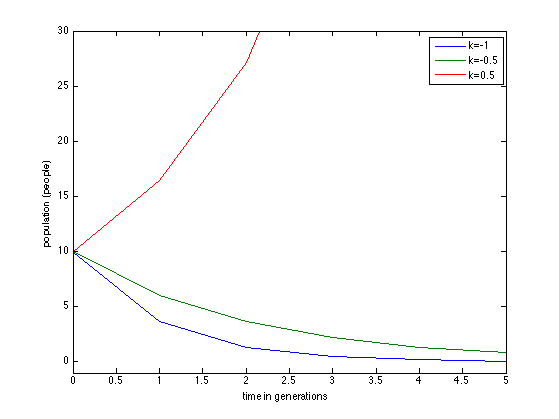
\includegraphics[width=\textwidth,height=0.7\textheight]{./exp_pop}
\end{figure}

\end{frame}

%%%%--------------------------------------------------------------------------------------------------------------------------------------------------------------------------------------------------------------------------%
\begin{frame}
\frametitle{More Graphs!}

We can now check more parameters! 

\begin{figure}
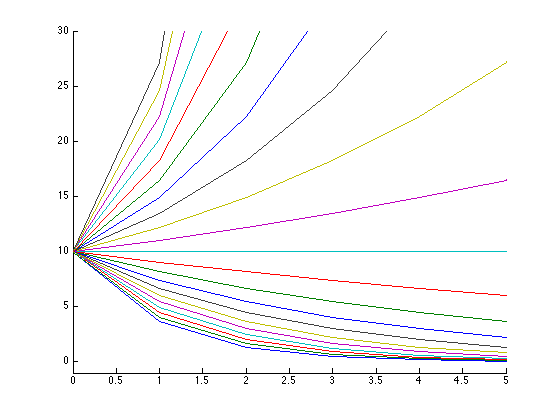
\includegraphics[width=\textwidth,height=0.7\textheight]{./exp_color}
\end{figure}

\end{frame}

%%%%--------------------------------------------------------------------------------------------------------------------------------------------------------------------------------------------------------------------------%
\begin{frame}
\frametitle{Modeling Epidemiology} 

{\tiny
Now we want to consider tracking a disease amongst a population of individuals. Ideas modeling this (\textcolor{red}{Simple example})
}
\begin{itemize}
\item People transfer from three states: Healthy $\rightarrow$ sick $\rightarrow$ healthy(immune). 
\item \textcolor{red}{What causes the transfer between the three states?} 
\pause 
\item Healthy people get sick when they interact with the sick, sick people become healthy again after medicine or a period of recover time. 
\item \textcolor{red}{What are the parameters and how do we want to denote each population?} 
\pause 
\item Healthy people = Susceptible ($\mathcal{S}$), sick = infected ($\mathcal{I}$), immune = removed population ($\mathcal{R}$) 
\item Parameters: Probability of getting sick: $\alpha$, chance at each time step of recovering (if sick): $\beta$, initial populations and total population $N$.
\item Questions: Are we adding people to the healthy population? Do immune people eventually return to susceptible? What time scale? 
\end{itemize}


\end{frame}

%%%%--------------------------------------------------------------------------------------------------------------------------------------------------------------------------------------------------------------------------%
\begin{frame}
\frametitle{Writing the Equations}

There are three quantities changing in time and depending on our choices previously will influence what the equations look like! \textcolor{red}{Write out your equations} 
\pause
\begin{align*}
\frac{d\mathcal{S}}{dt} &= -\frac{\alpha}{N}\mathcal{S}\mathcal{I}\\
\frac{d\mathcal{I}}{dt} &= \frac{\alpha}{N}\mathcal{S}\mathcal{I} - \beta\mathcal{I}\\
\frac{d\mathcal{R}}{dt} &= \beta\mathcal{I}
\end{align*}

What are some parameters in this system? \textcolor{red}{Brainstorm!} How do we make this model better? \textcolor{red}{Brainstorm!}

\end{frame}


%%%%--------------------------------------------------------------------------------------------------------------------------------------------------------------------------------------------------------------------------%

\begin{frame}
\frametitle{Homework}
{\tiny
For the current epidemiology model: 
}
\begin{itemize}

\item Identify important parameter values of $\alpha$ and $\beta$. What long term solutions are possible with these parameters? Does population size matter? 
\item Compute the two parameter values from a real world scenario (choose a disease and do a bit of research on it) 
\item Explain what is wrong with the model, are there long term solutions which can't be obtained? 
\item \textcolor{red}{Develop a new system with the following characteristics: }

\begin{itemize}
\item Recovered population has a very slight chance of becoming susceptible again. Define the parameter value which controls this and discuss how this changes the long term behavior of the system. 
\item Add an immunized population which susceptible can change to, should they be completely removed?. Complete the above tasks for this new population. 
\item Add birth to the susceptible population, make the frequency be relevant to your time scales. How does this change the outcome? 
\end{itemize} 
\end{itemize}

\end{frame}

%%%%--------------------------------------------------------------------------------------------------------------------------------------------------------------------------------------------------------------------------%


\end{document}
